

\documentclass{beamer}
\usepackage{multicol}
\usepackage{graphicx}
\usepackage{caption}
\usepackage[absolute,overlay]{textpos}   % for adding floats anywhere on the slide
\usepackage{amsmath}
\usepackage{pifont}
\usepackage{fontawesome}
\usepackage{epstopdf}                     % for using .eps figures
%%% A to-do list 
\newcommand{\future}{\faStarO}
\newcommand{\cmark}{\ding{51}}%
\newcommand{\xmark}{\ding{55}}%
\newcommand{\todo}{$\square$}{\raisebox{2pt}}
%\newcommand{\future}{\todo}
\newcommand{\done}{\rlap{$\square$}{\raisebox{2pt}{\large\hspace{1pt}\cmark}}%
    \hspace{-2.5pt}}
\newcommand{\wontfix}{\rlap{$\square$}{\large\hspace{1pt}\xmark}}

% There are many different themes available for Beamer. A comprehensive
% list with examples is given here:
% http://deic.uab.es/~iblanes/beamer_gallery/index_by_theme.html
%\usetheme{AnnArbor}
%\usetheme{Antibes}
%\usetheme{Bergen}
%\usetheme{Berkeley}
%\usetheme{Berlin}
\usetheme{Boadilla}
%\usetheme{boxes}
%\usetheme{CambridgeUS}
%\usetheme{Copenhagen}
%\usetheme{Darmstadt}
%\usetheme{default}
%\usetheme{Frankfurt}
%\usetheme{Goettingen}
%\usetheme{Hannover}
%\usetheme{Ilmenau}
%\usetheme{JuanLesPins}
%\usetheme{Luebeck}
%\usetheme{Madrid}
%\usetheme{Malmoe}
%\usetheme{Marburg}
%\usetheme{Montpellier}
%\usetheme{PaloAlto}
%\usetheme{Pittsburgh}
%\usetheme{Rochester}
%\usetheme{Singapore}
%\usetheme{Szeged}
%\usetheme{Warsaw}

%%% Set up image path %%%
\graphicspath{ {figures/} }

%%% Prettier + sign for Foldon+ScafFold
\def\Plus{\texttt{+}}

%%% New symbol 
\newcommand{\new}{%
  \begin{textblock*}{2cm}(11cm,0cm) % {block width} (coords)

\includegraphics[width=2cm]{new.png}
\end{textblock*}
}

\title[Short title]{This is a big title}

% A subtitle is optional
\subtitle{Sometimes I like a subtitle too}

\author[Clare E. West]{Clare E. West\inst{1,2}, Saulo H.P. de Oliveira\inst{3,4} \& Charlotte M. Deane\inst{2}  }

% - Give the names in the same order as the appear in the paper.
% - Use the \inst{?} command only if the authors have different
%   affiliation.

\institute[University of Oxford] 
{
  SABS CDT\\
  University of Oxford}
  
\institute[]
{\tiny \inst{1} 
	SABS CDT \\
	University of Oxford
	\and
 \inst{2} 
 	Department of Statistics \\
 	University of Oxford
 	\and
  \inst{3}
  SLAC National Accelerator Laboratory \\
  Stanford University 
  \and
 \inst{4}
 	Bioengineering \\
  Stanford University}

\begin{document}

\date{April 2019}

\begin{frame}
  \titlepage
\end{frame}


\section{Introduction}

\begin{frame}{Template-Free Protein Structure Prediction}
  \begin{itemize}
\setlength\itemsep{1em}  % change space between items
\item Current structure prediction heuristics are limited by the enormous conformational search space
\item Proteins adopt their native structures \textit{in vivo} by searching  conformational space very efficiently
\item Biologically-inspired sequential prediction has improved protein structure prediction
\item Blah blah   
\end{itemize}
\end{frame}


%\tiny{Englander, S.W., Mayne, L., 2014. The nature of protein folding pathways. Proc. Natl. Acad. Sci. U. S. A. 111, 15873–80.}


\begin{frame}{Figure-on-top slide example}
  \new
  \centering
  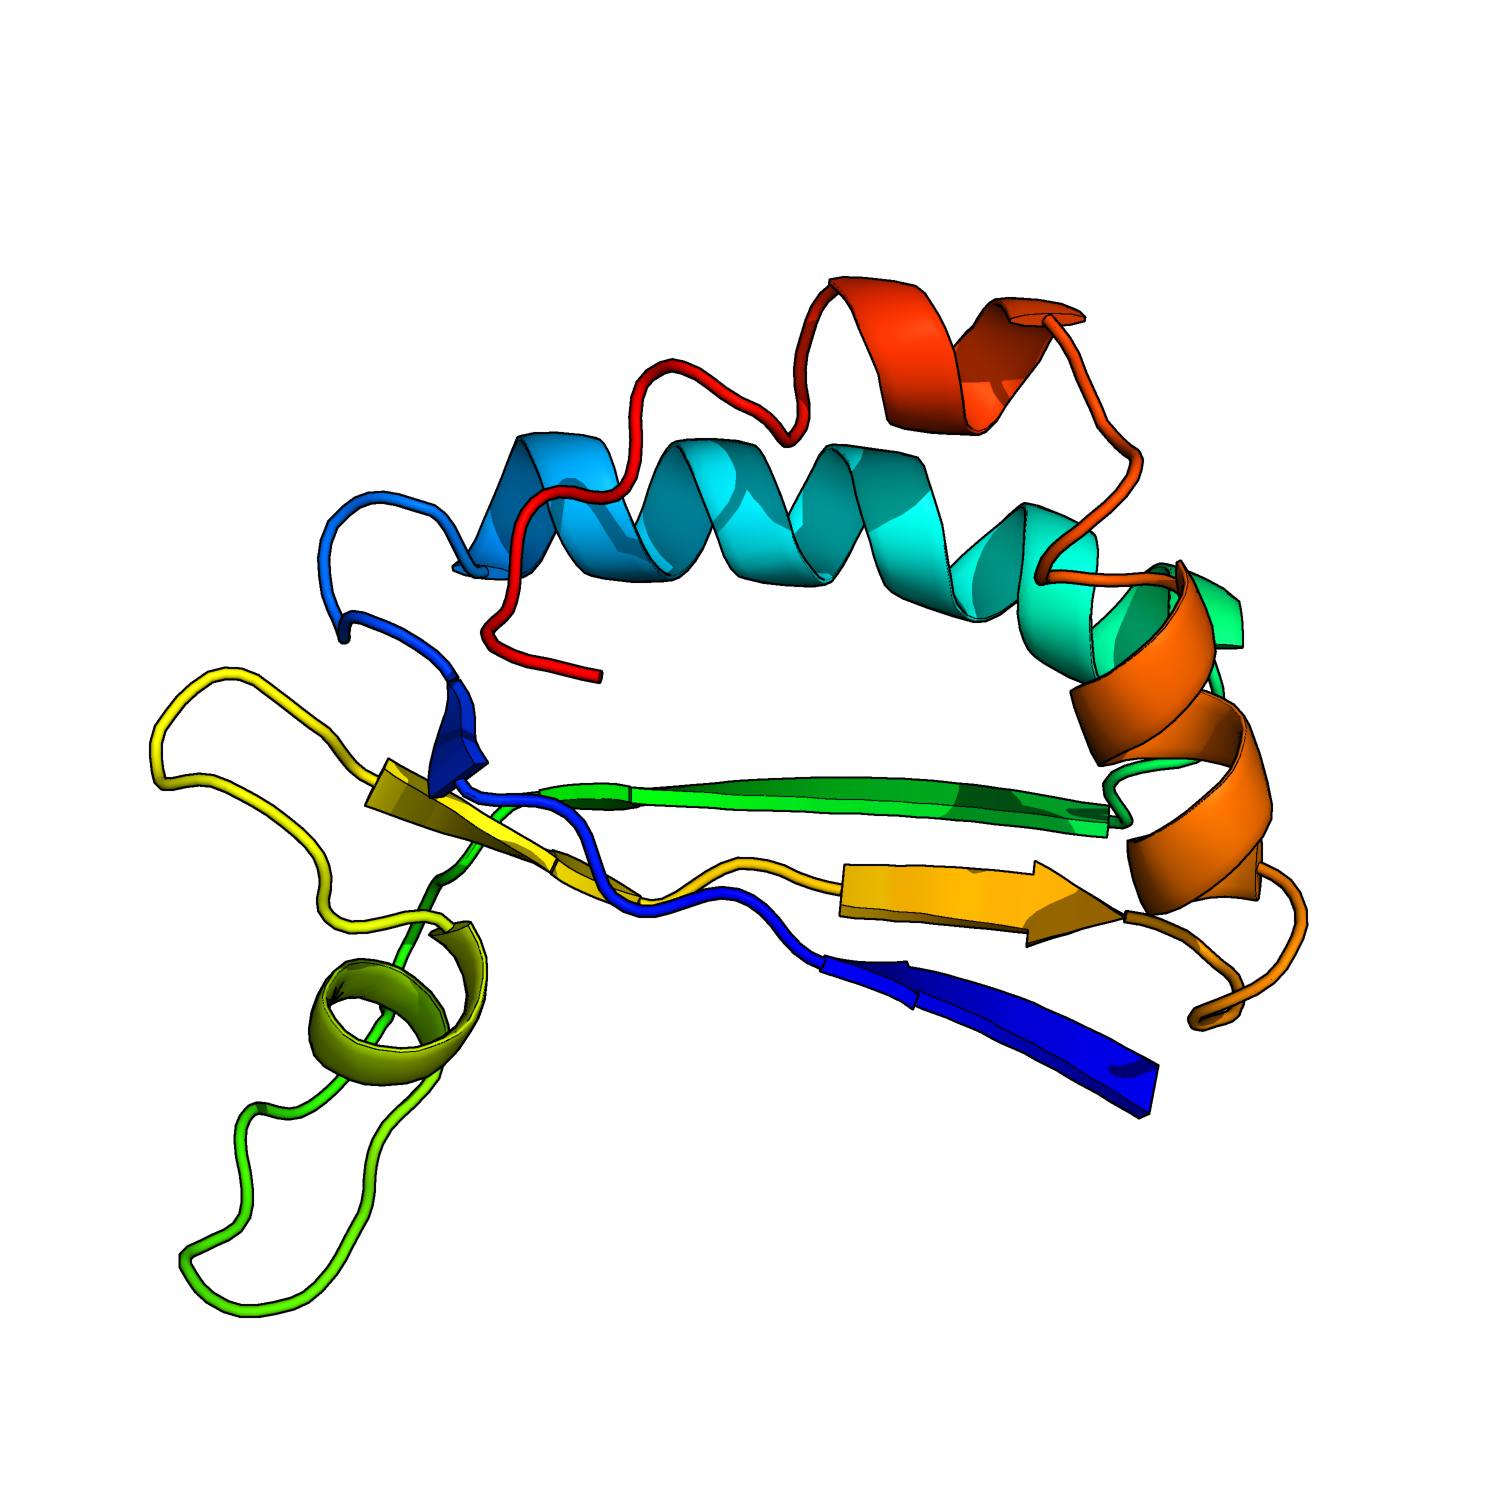
\includegraphics[width=0.5\textwidth]{2OKQA.png}
  \begin{itemize}
    \item On this slide, the figure is on top and the text is underneath 
    \item This is also an example of the new label for exciting new things
  \end{itemize}
\end{frame}

\begin{frame}{Figure on one side slide example}
  \begin{columns}
    \begin{column}{0.5\textwidth}
      \centering
      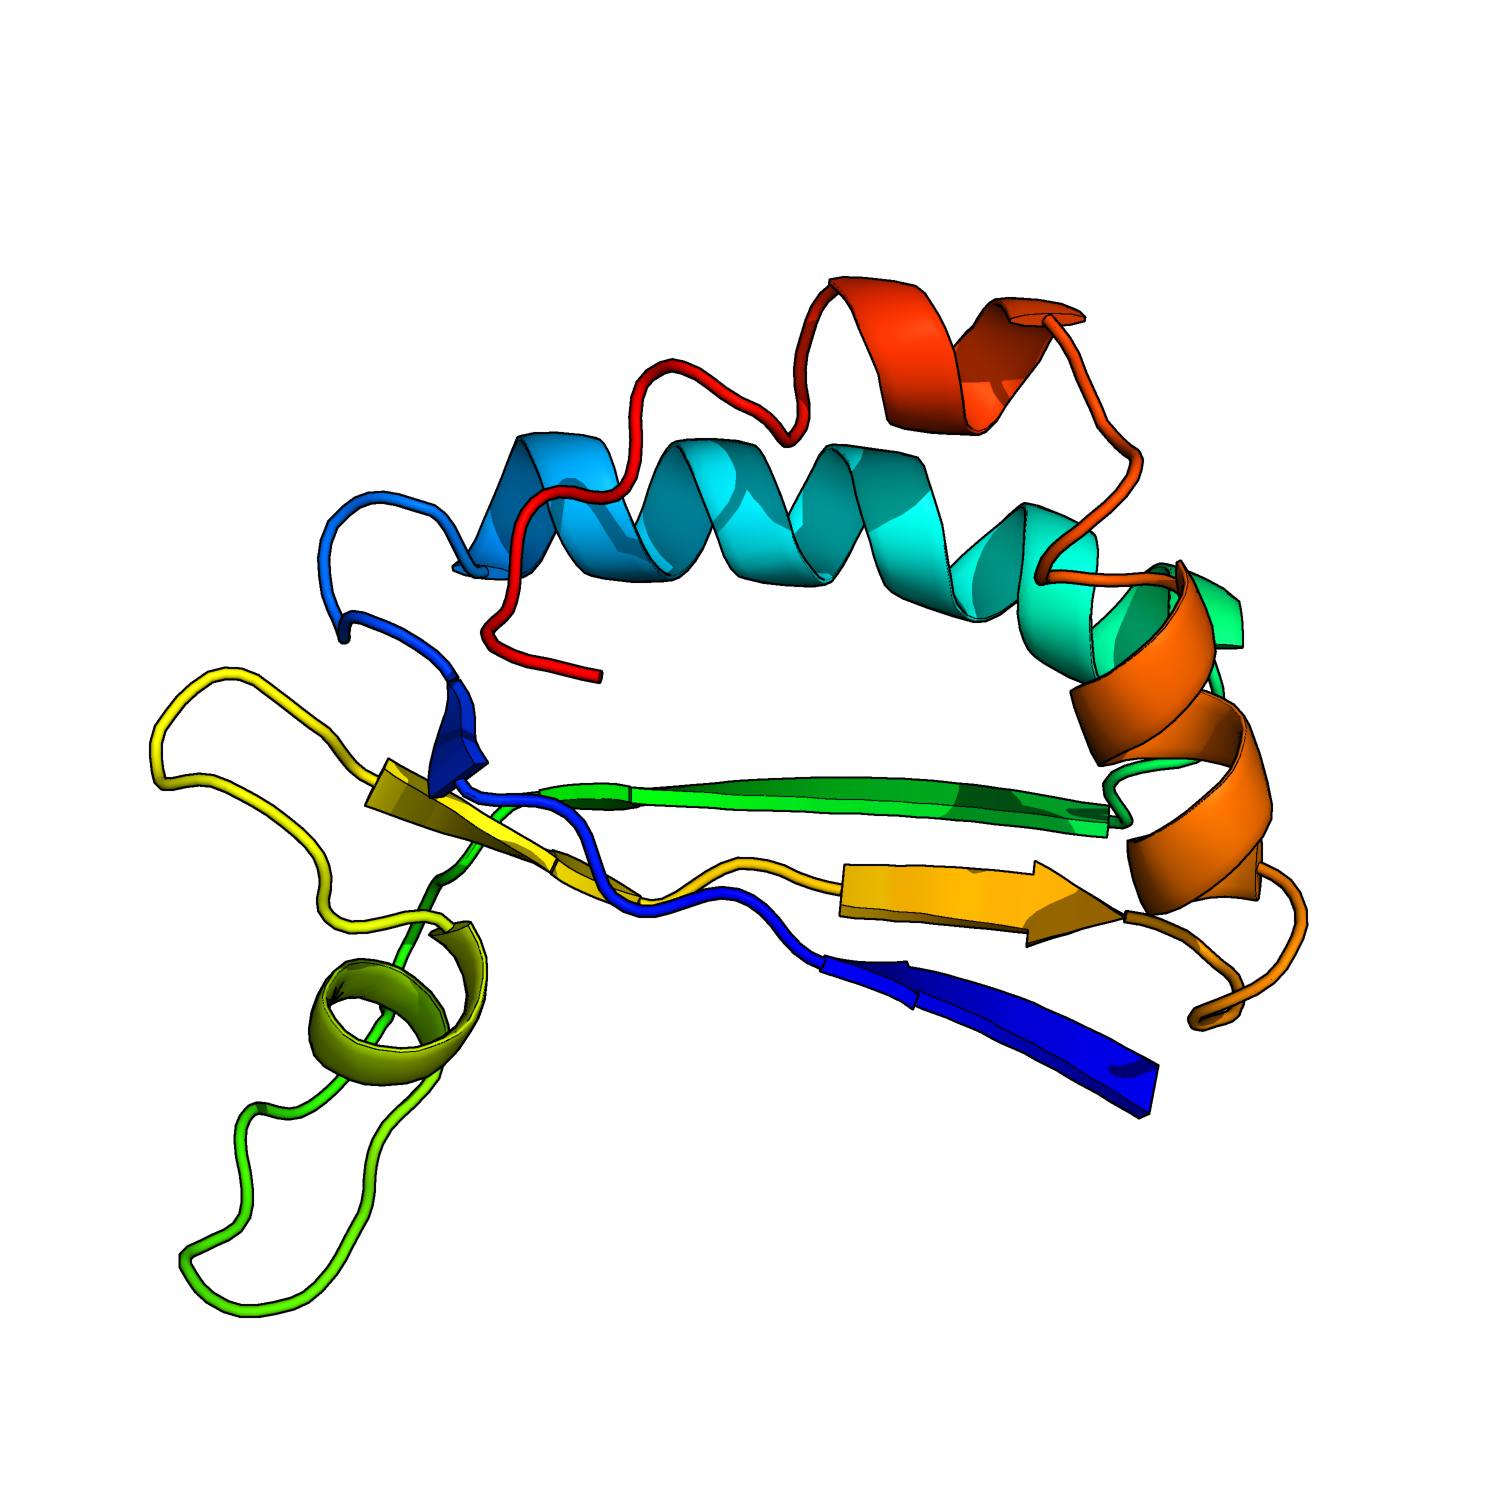
\includegraphics[width=1\textwidth]{2OKQA.png}
    \end{column}
    \begin{column}{0.5\textwidth}
      \begin{itemize}
      \setlength{\itemsep}{1em}
        \item This text is to the right of the figure 
        \begin{itemize}
          \item Wow look at that structure  
          \item Over there on the left
          \item I like it 
          \item Very nice 
        \end{itemize}
        \item Models are ranked and grouped into confidence categories
      \end{itemize}
    \end{column}
  \end{columns}
\end{frame}


\begin{frame}{Block slide example}
\vspace{5mm}
  \begin{block}{Block title}
    \begin{columns}
      \begin{column}{0.45\textwidth}
  \begin{itemize}
  \setlength{\itemsep}{1em}
    \item I'm partial to a block slide:
      \begin{itemize}
        \item To be honest 
        \item I don't know why
        \item I just like it 
        \item sometimes
      \end{itemize}
    \item Models are ranked and grouped into confidence categories
  \end{itemize}
\end{column}
\begin{column}{0.5\textwidth}
  \centering
  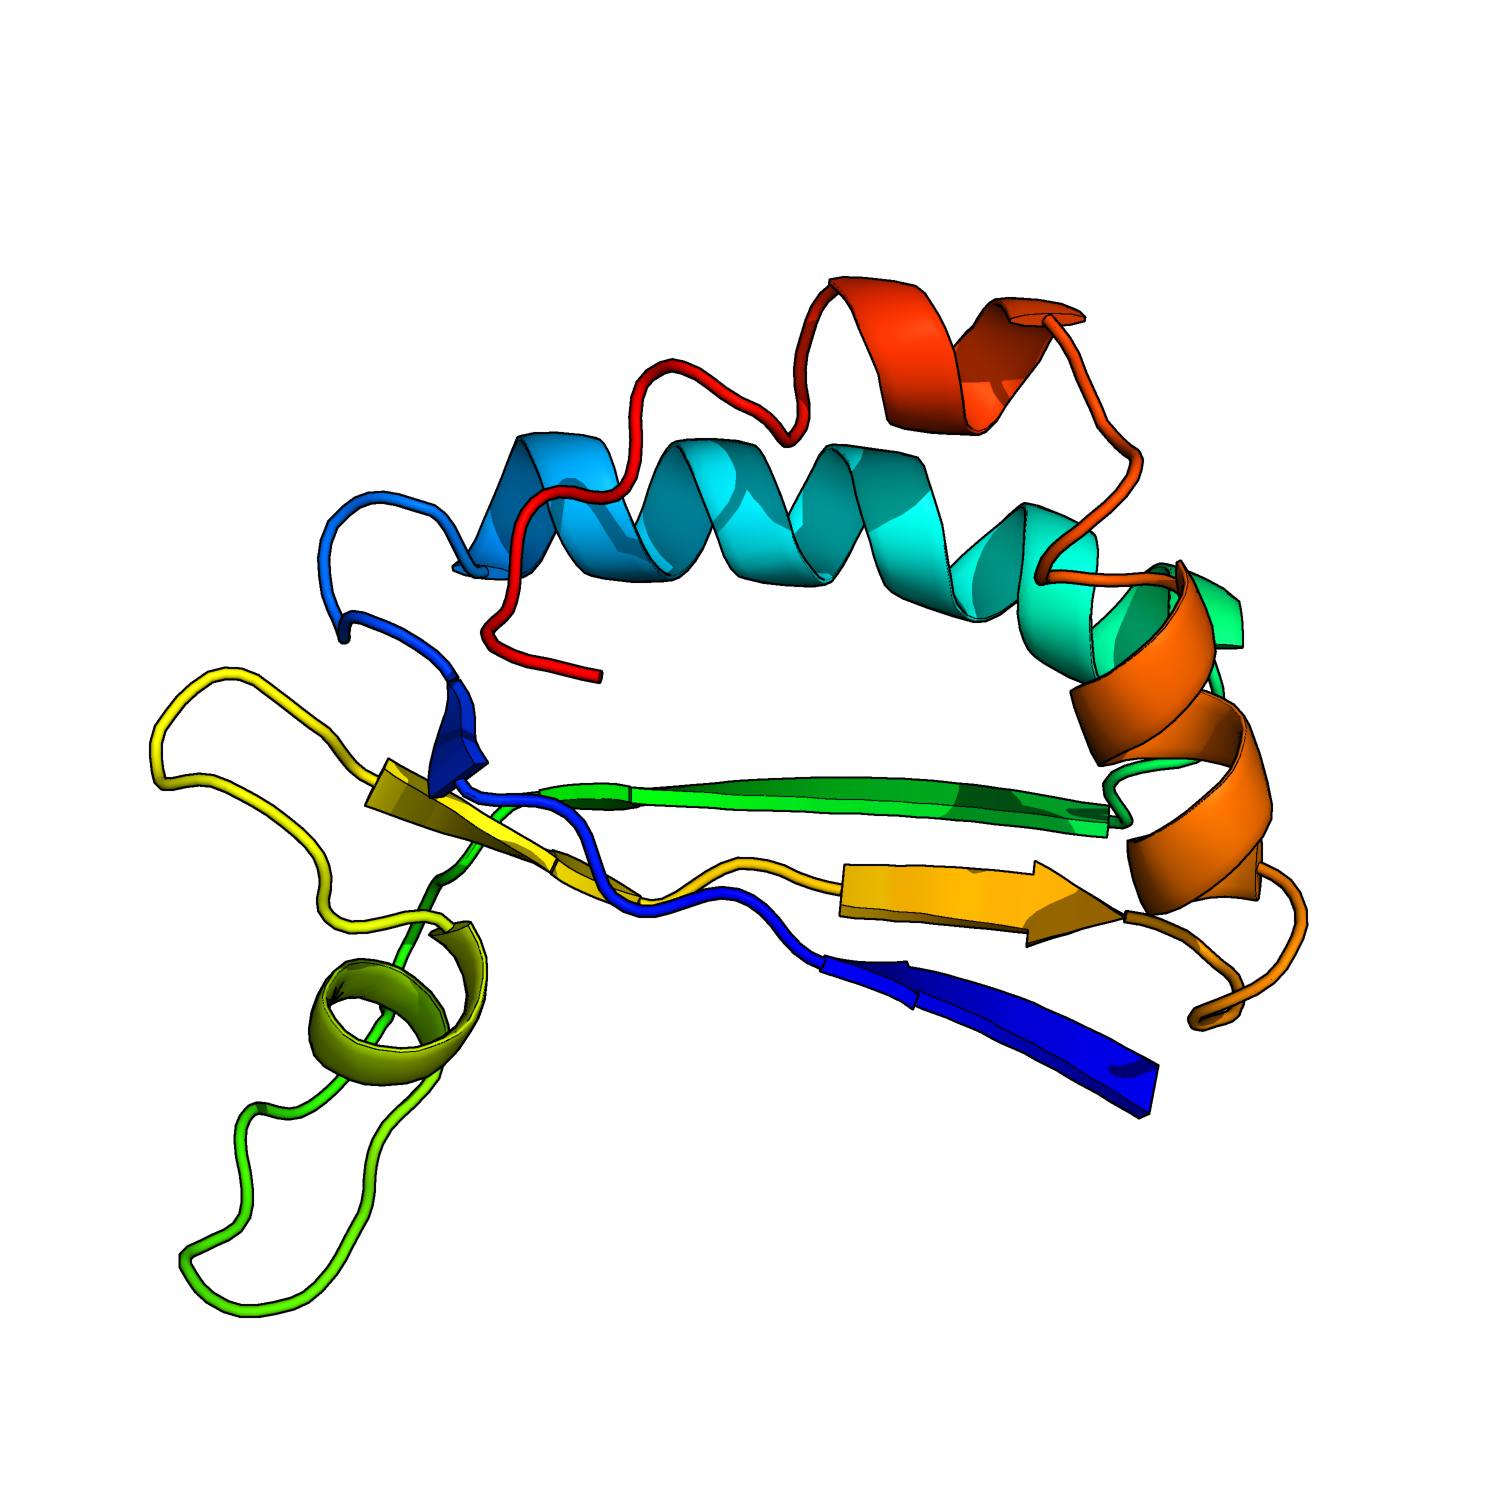
\includegraphics[width=0.9\textwidth]{2OKQA.png}
\end{column}
\end{columns}
\end{block}
\vspace{10mm}
\tiny{Include citations like this, if I need them. For example this structure is 2OKQA }

\end{frame}

\begin{frame}{Protocol and set of example cases}
  \new
  \begin{itemize}
    \item Slide for presenting examples of targets or models 
      \begin{itemize}
        \item Some details in case I need them % ($\leq$2.5\AA)
      \end{itemize}
    \item Some more details about the structures 
    \item Validation: aligned RMSD ($\leq$5\AA) and minimised RMSD ($\leq$2.5\AA) of sampled region
  \end{itemize}
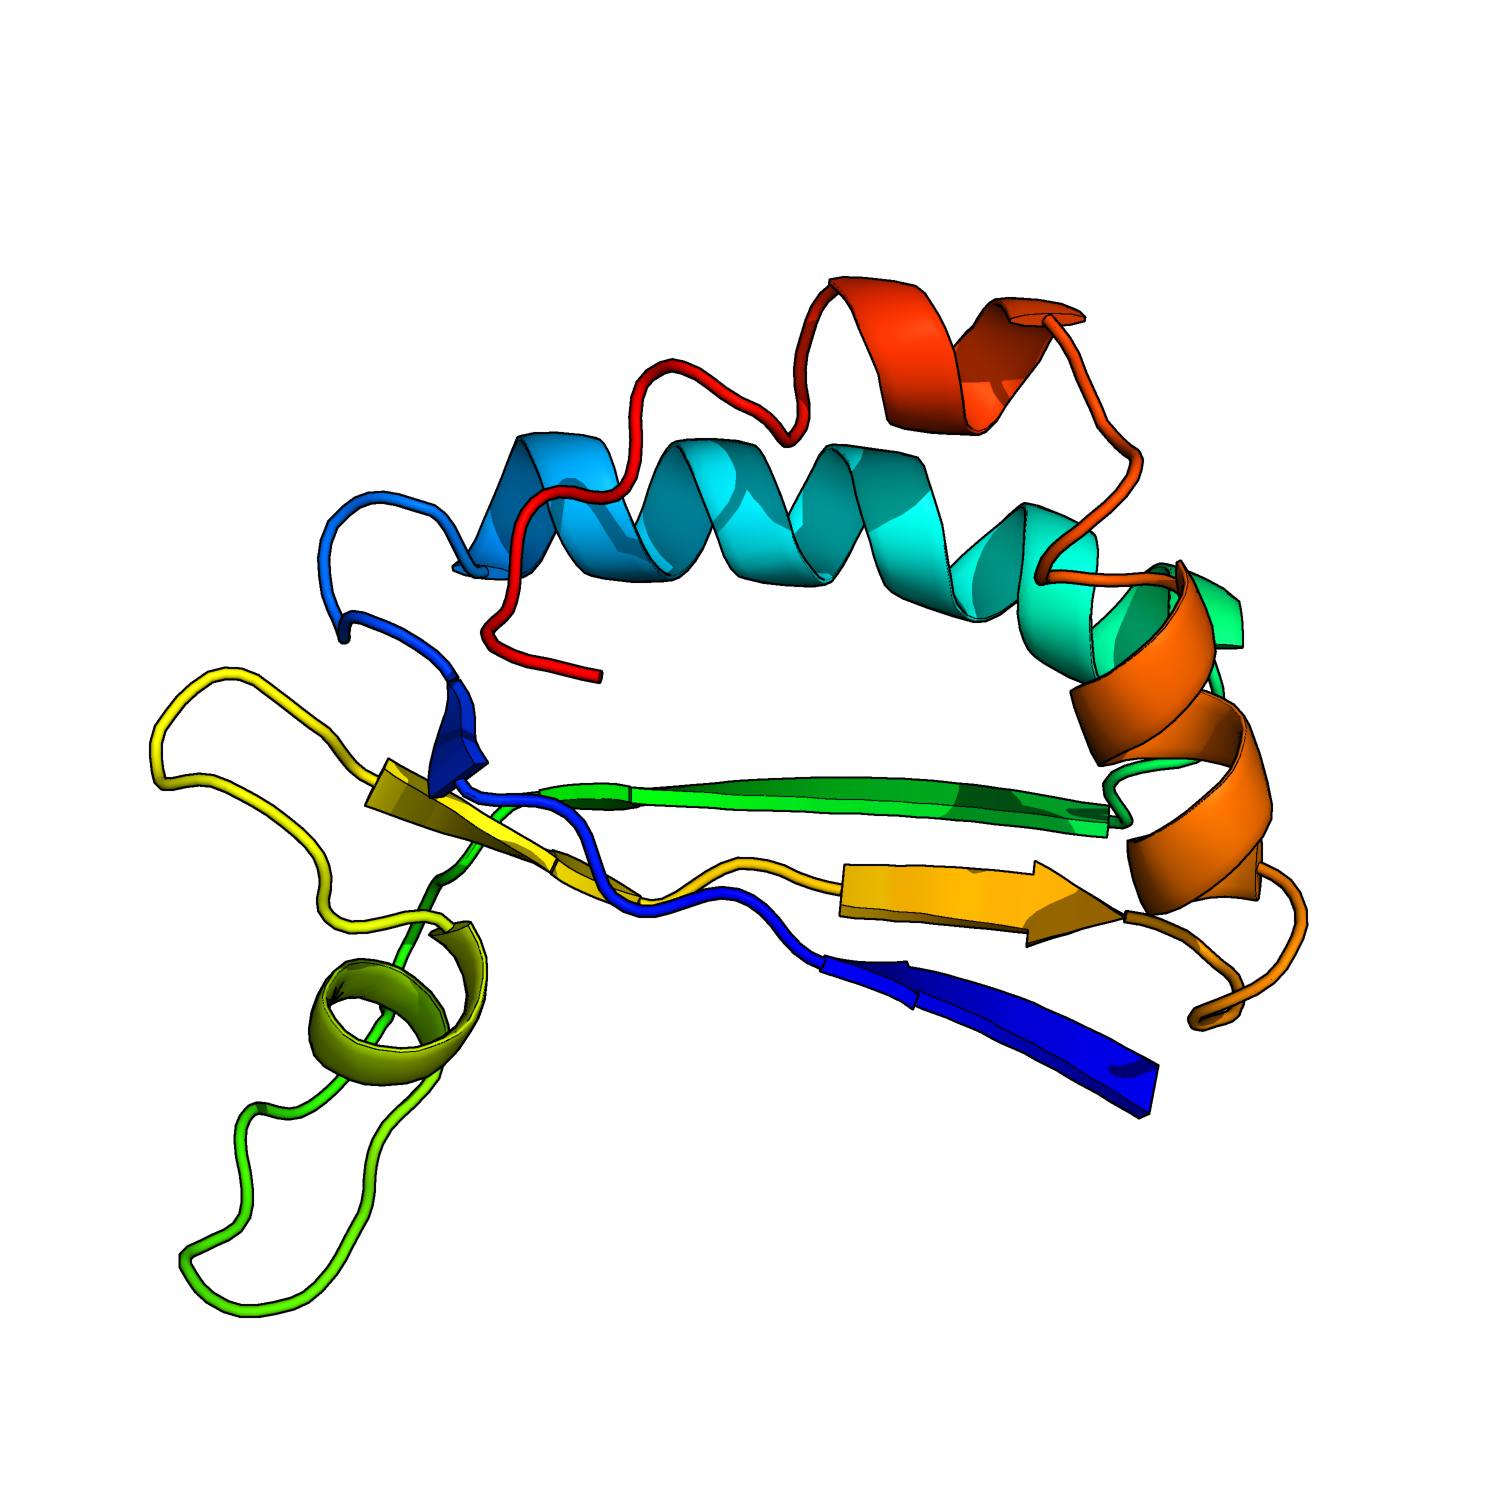
\includegraphics[width=0.2\textwidth]{2OKQA.png}
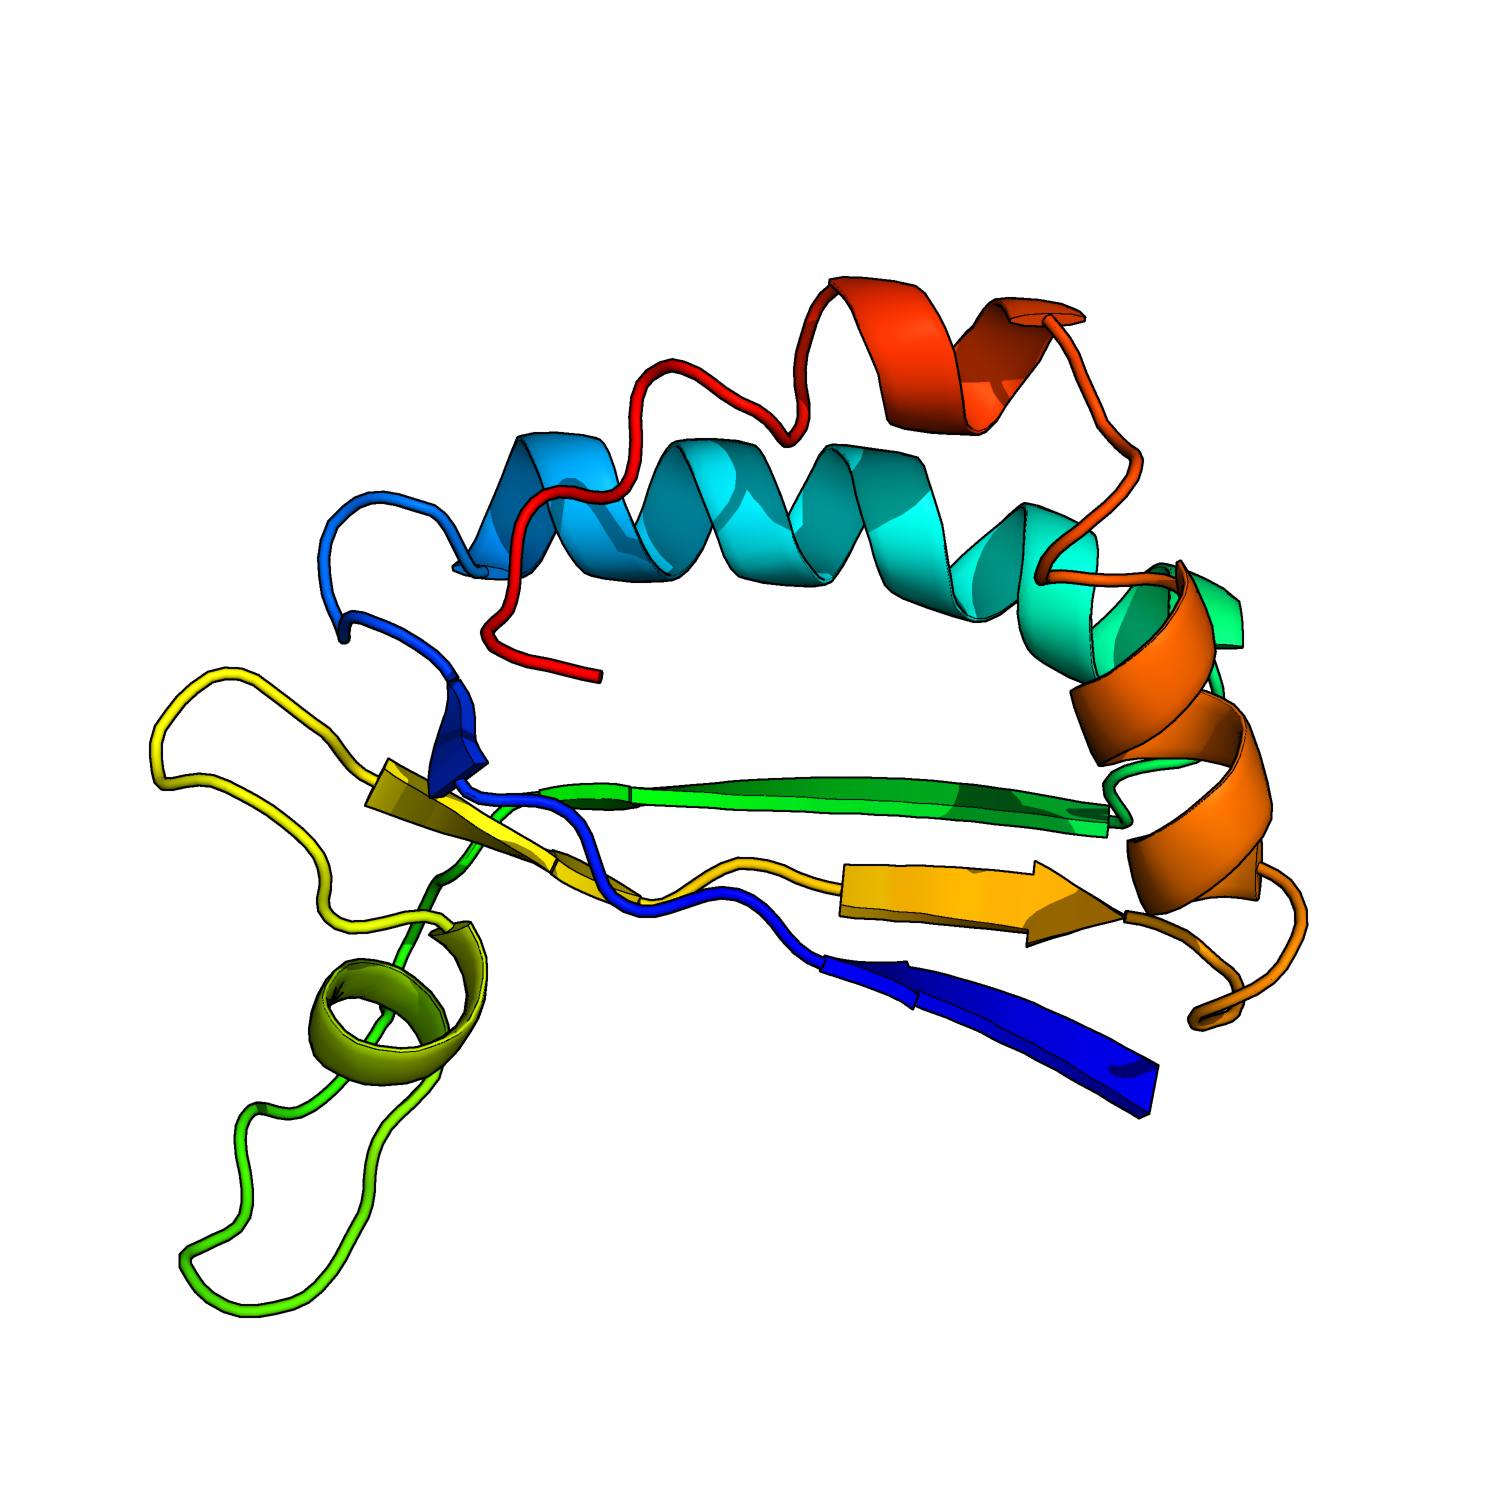
\includegraphics[width=0.2\textwidth]{2OKQA.png}
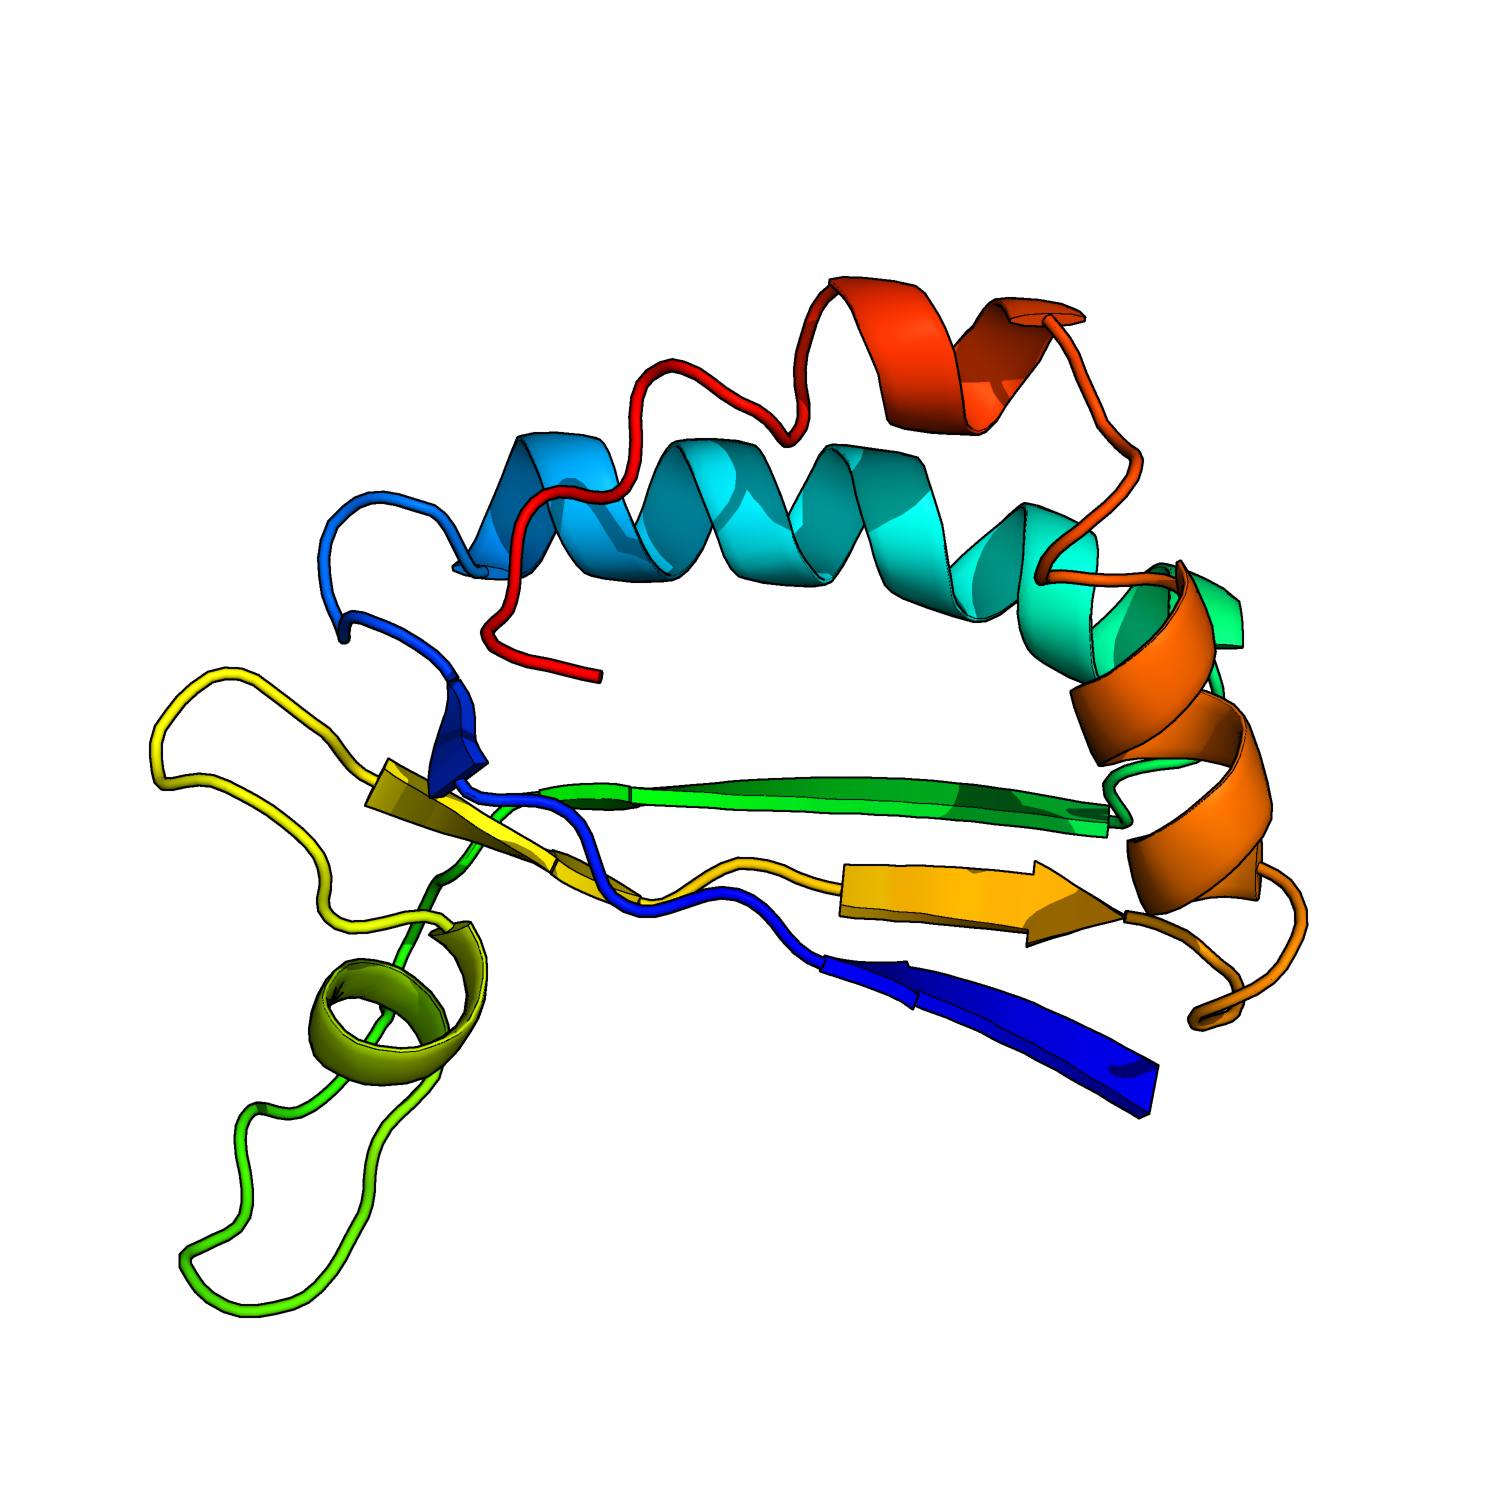
\includegraphics[width=0.2\textwidth]{2OKQA.png}
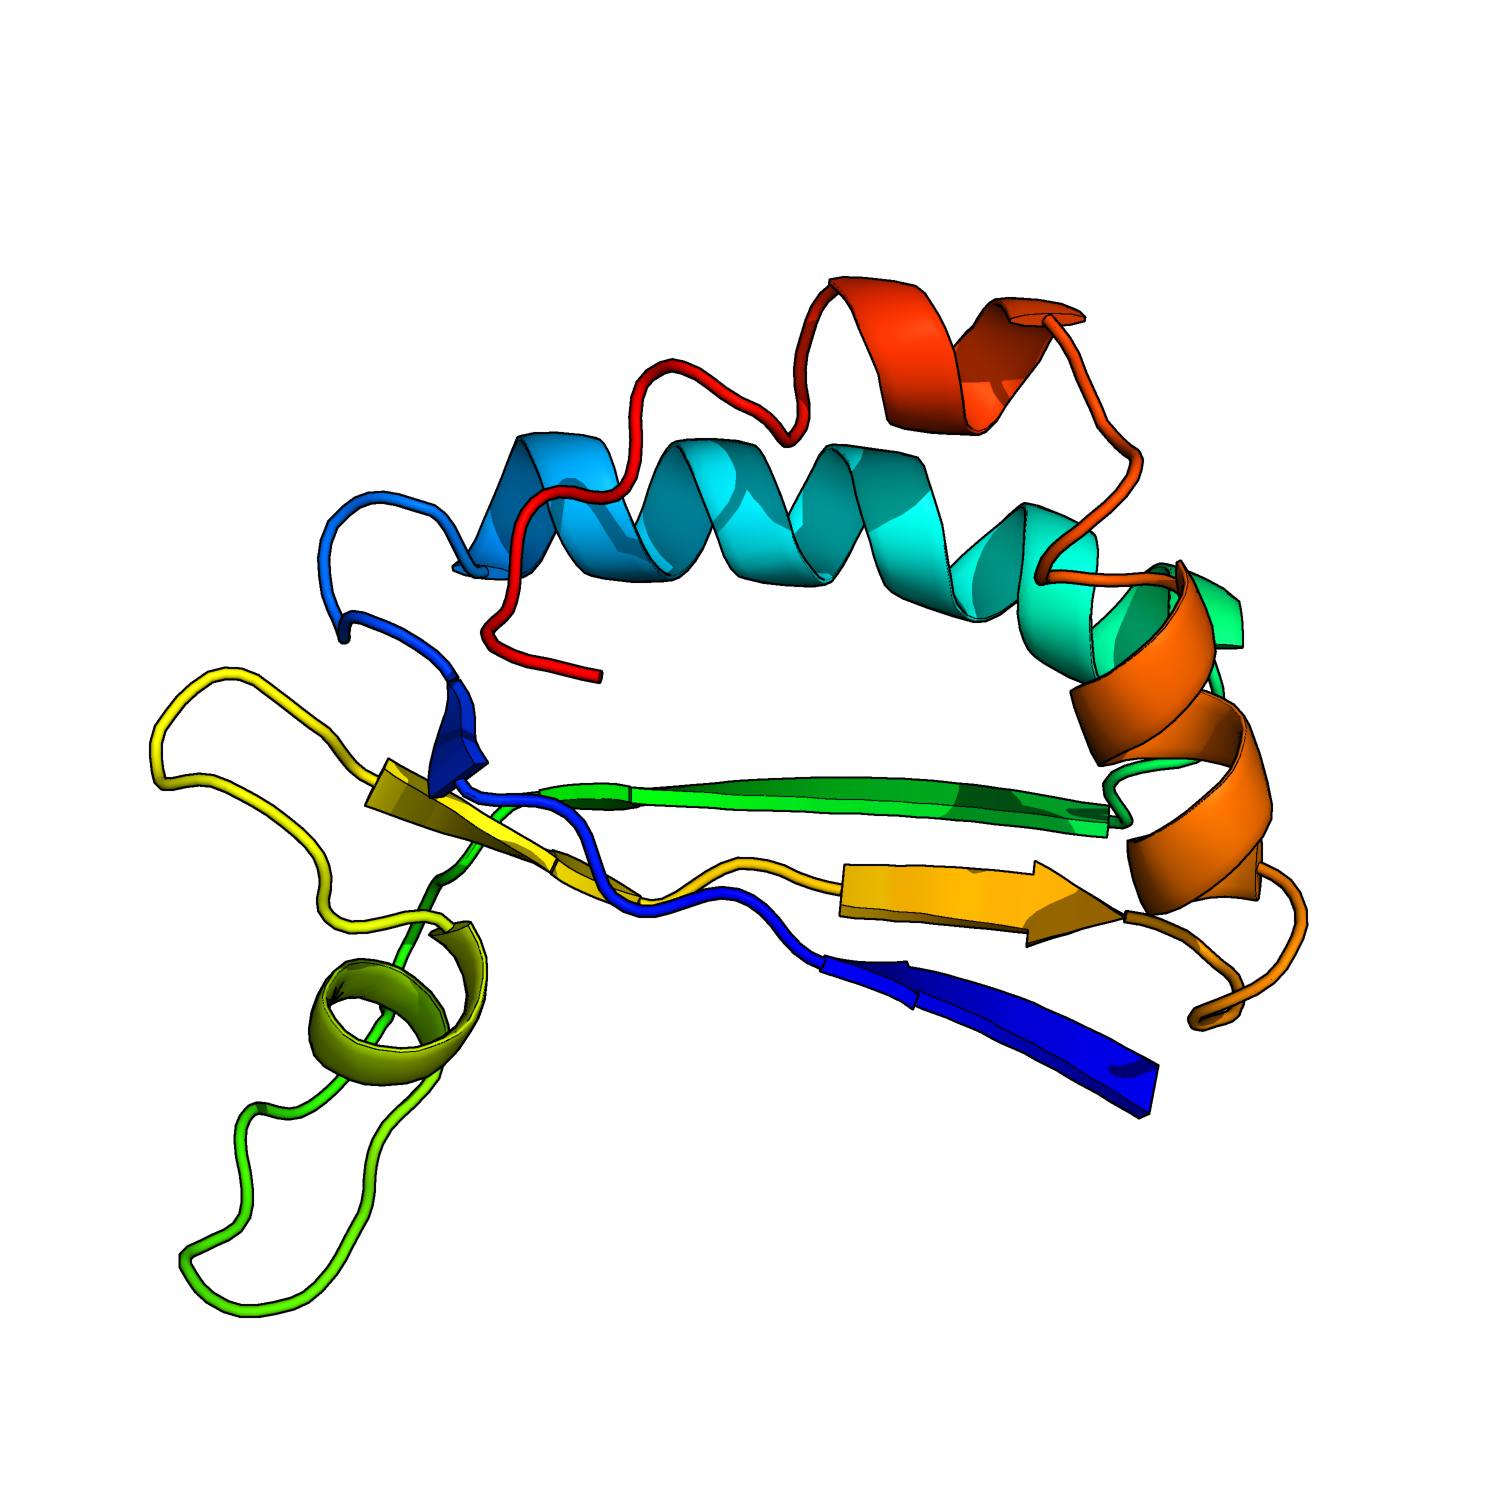
\includegraphics[width=0.2\textwidth]{2OKQA.png}
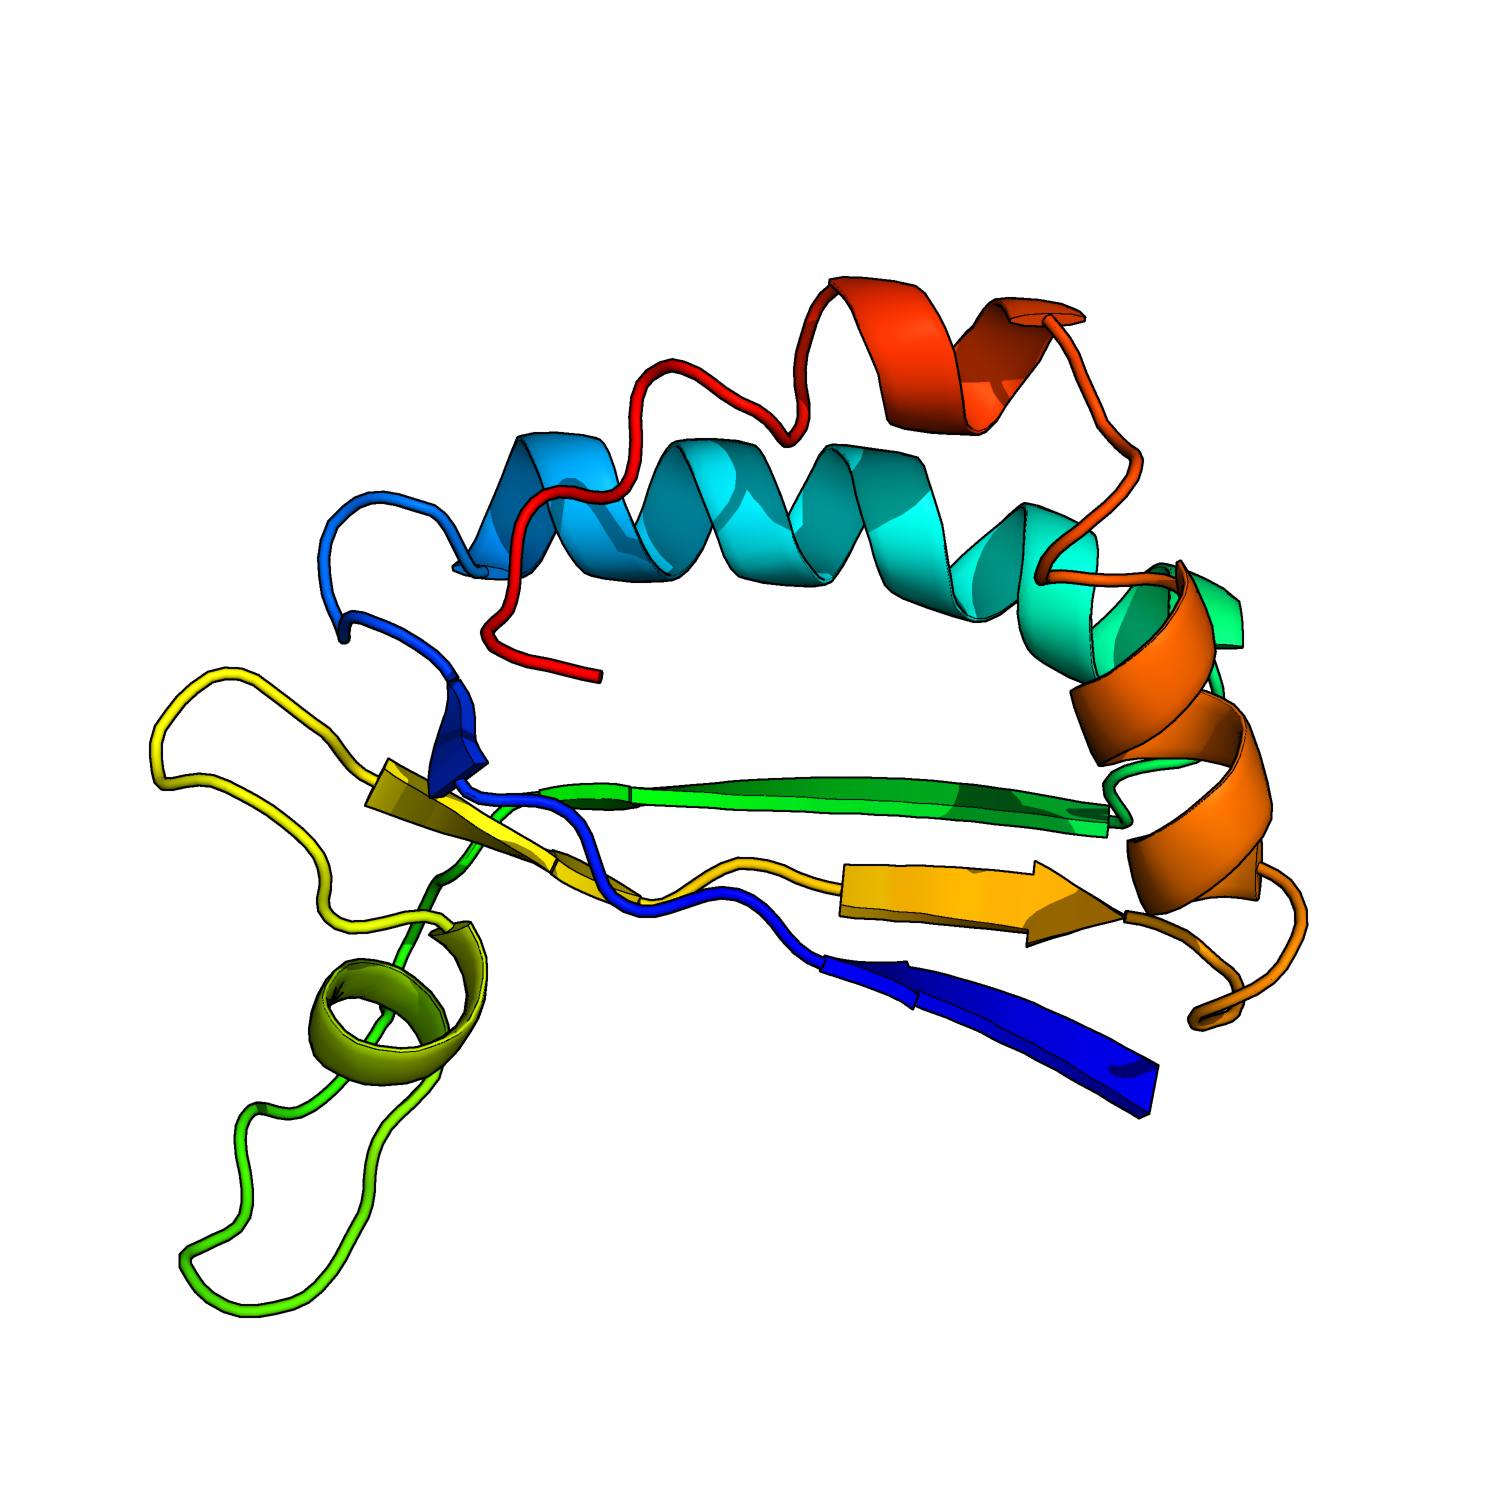
\includegraphics[width=0.2\textwidth]{2OKQA.png}

\small \hspace{15pt} 2.32, 1.99 \hfill 9.56, 8.58 \hfill 11.20, 8,16 \hfill 2.67, 1.75 \hfill 6.05, 3.48  \hspace{15pt}

\small \hspace{25pt} Good  \hfill    Bad  \hfill   Bad  \hfill   Good  \hfill   Okay \hspace{25pt}
\end{frame}

\section{Foldon\Plus ScafFold: Stepwise prediction of long and multidomain proteins}
\begin{frame}{Foldons and Protein Folding}
  \begin{center}
    \begin{block}{The Foldon Hypothesis}
      \begin{itemize}
        \item \textbf{Foldons: small, separately cooperative units}
        \item Folding occurs via an ordered process of foldon-determined steps, in which formed foldons guide and stabilise the next foldons  
      \end{itemize}
      \begin{columns}
        \begin{column}{0.5\textwidth}
          \begin{itemize}
            \item Foldons are...
              \begin{itemize}
                \item small enough to overcome the Levinthal time scale problem
                \item large enough to provide the energy bias to drive folding 
              \end{itemize}
          \end{itemize}
        \end{column}
        \begin{column}{0.5\textwidth}
          \begin{center}
            \includegraphics[width=0.8\textwidth]{/Users/clarewest/Start2Fold/foldons}\\
          \end{center}
        \end{column}
      \end{columns}
      \vspace{3mm}
    \end{block}
    \vspace{0.5mm}
  \end{center}
    \tiny{Jeng, M.F., Englander, S.W., 1991. Stable submolecular folding units in a non-compact form of cytochrome c. J. Mol. Biol. 221, 1045–61.} \\
    \tiny{Maity, H., Maity, M., Walter Englander, S., 2004. How cytochrome c folds, and why: Submolecular foldon units and their stepwise sequential stabilization. J. Mol. Biol. 343, 223–233.} \\
    \tiny{Hu, W., Kan, Z.-Y., Mayne, L., Englander, S.W., 2016. Cytochrome c folds through foldon-dependent native-like intermediates in an ordered pathway. Proc. Natl. Acad. Sci. U. S. A. 113, 3809–14.} \\
\end{frame}

\begin{frame}{To do list}
  \centering
  \begin{itemize}
      \setlength\itemsep{1.5em}
    \item Big difficult task 
    \begin{itemize}      \setlength\itemsep{1em}
      \item[\done] A task I've completed already  
      \item[\done] Another task I've completed already
      \item[\todo] A task I haven't completed 
      \item[\todo] A task I haven't completed 
    \end{itemize}
    \item Another related big difficult task on the same topic 
    \begin{itemize}      \setlength\itemsep{1em}
      \item[\done] Something that I've already done  
      \item[\done] Something that I haven't yet done 
      \item[\future] Something that I would do in my dreams 
    \end{itemize}
  \end{itemize}
\end{frame}

\section{Conclusion}

\begin{frame}{Ackowledgements}
\centering

\includegraphics[width=0.8\textwidth]{UpdatedSABSLogo1}


\includegraphics[width=0.1\textwidth]{UCB}\\
\end{frame}



\end{document}


